\documentclass{article}
\setlength{\parindent}{0pt}
\setlength{\parskip}{2ex plus 0.5ex minus 0.2ex}
\usepackage[margin=1in]{geometry}
\usepackage{graphicx}
\usepackage{hyperref}
\usepackage{cleveref}
\usepackage{textcomp}
\usepackage{placeins}
\usepackage[T1]{fontenc}
\usepackage{gensymb}
\usepackage[utf8]{inputenc}
\graphicspath{{./figures/}}

\title{Advanced Reactor Fuel cycle Molten Salt Reactor Design}
\author{Alexander Lindsay, Katy Huff} % As you author additions/changes, add
                                      % your name here!!!

% To do: Decide how to present figures in a way that they don't have both our
% figure labels as well as the original documents; also make sure we are
% reproducing those figures in an ethical way

\begin{document}
\maketitle

\section{Brief History}

The basis for this quick synopsis comes from
\cite{wiki:Molten_salt_reactor}. Research into molten salt reactors (MSRs) began
in earnest with the Aircraft Reactor Experiment (ARE), with experiments shared
between Oak Ridge National Lab (ORNL) and what is now Idaho National Lab
(INL). The ARE used NaF-ZrF$_4$-UF$_4$ (53-41-6 mol\%) as fuel. The reactor was
moderated by beryllium oxide (BeO), used liquid sodium as the secondary coolant,
and had a peak tempeature around 860 \textdegree C. The ARE managed to generate
100 MWh over the course of nine days in 1954. There was another reactor that
went critical at ORNL in 1957 called the Pratt and Whitney Aircraft Reactor-1
(PWAR-1). Although it produced essentially no power, the PWAR-1 is still one of
only three critical MSRs ever built.

The most successful MSR was the Molten-Salt Reactor Experiment (MSRE) which went
critical in 1965 and operated for four years at ORNL. The MSRE fuel was
LiF-BeF$_2$-ZrF$_4$-UF$_4$ (65-29-5-1 mol\%) with graphite core moderation. The
secondary coolant was 2LiF-BeF$_2$ (also known as FLiBe). Operating temperatures
went as high as 650 \textdegree C. MSRE neutronics were meant to mimic that of
an epithermal thorium molten salt breeder reactor (MSBR); however, for the MSRE
the expensive breeding blanket was sacrificed in favor of neutron
measurements. At full design power, the MSRE operated at 7.4 MW$_{th}$. Over the
course of the late 1960s the MSRE operated at full capacity for an equivalent of
1.5 years.

The logical follow-on from the MSRE was the MSBR; however, the MSBR was never
constructed. Funding for the MSR program was cut in favor of the liquid metal
fast-breeder reactor (LMFBR) program. Consequently, as of today, the ARE,
PWAR-1, and MSRE are the only critical MSRs ever operated.

\section{MSRE}

\subsection{Salt properties}

\begin{figure}[htpb]
  \centering
  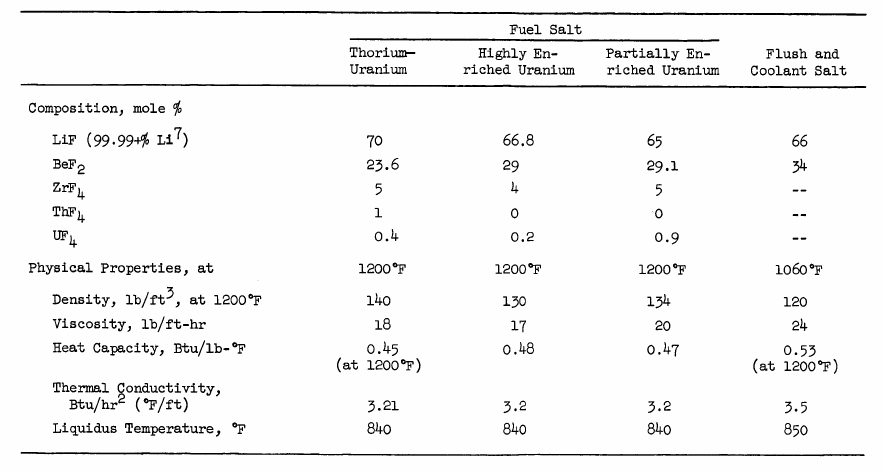
\includegraphics[width=\textwidth]{salt_properties.png}
  \caption{Composition and properties of fuel, flush, and coolant
    salts. \cite{robertson_msre_1965}}
  \label{fig:salt_properties}
\end{figure}

\subsection{Layout \& Equipment}

\begin{figure}[htpb]
  \centering
  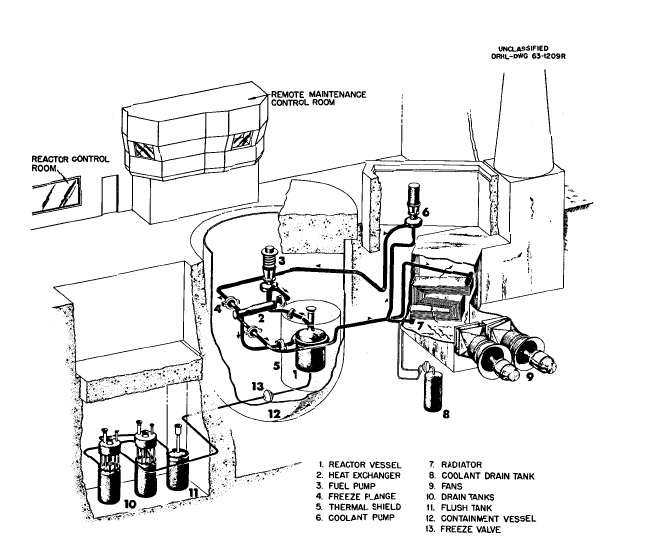
\includegraphics{flow_diagram.png}
  \caption{Macroscopic layout of the MSRE \cite{robertson_msre_1965}}
  \label{fig:MSRE_layout}
\end{figure}

\subsubsection{Reactor vessel}

\begin{figure}[htpb]
  \centering
  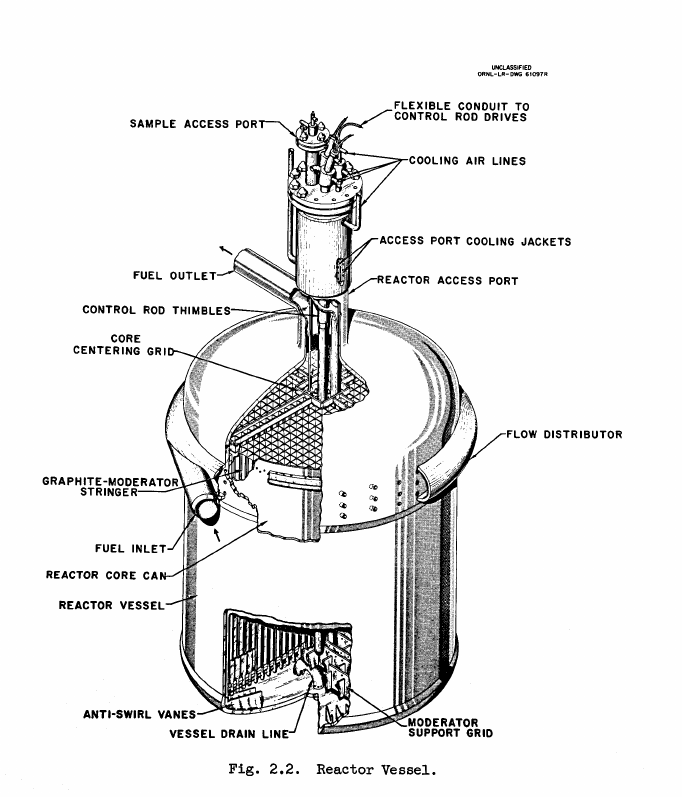
\includegraphics{MSRE_reactor_vessel.png}
  \caption{MSRE reactor vessel. \cite{robertson_msre_1965}}
  \label{fig:MSRE_reactor}
\end{figure}

\subsection{Reactivity considerations}

The MSRE has a negative temperature coefficient of 6.4 - 9.9 x $10^{-5}$
($\Delta$k/k)/\textdegree F depending on the choice of
fuel. \cite{robertson_msre_1965} The MSRE's three control rods have a combined
worth of 5.6 - 7.6 \% $\Delta$k/k, again depending on the
fuel. \cite{robertson_msre_1965}

\begin{figure}[htpb]
  \centering
  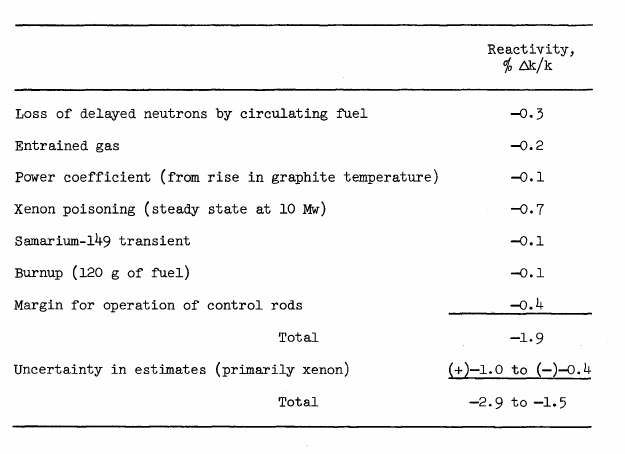
\includegraphics{reactivity-losses.png}
  \caption{Losses in reactivity associated with different
    phenomena. \cite{robertson_msre_1965}}
  \label{fig:reactivity_losses}
\end{figure}

\section{MSRE adaption for modelling}

\subsection{Kophazi article review}

Kophazi developed a 3D time-dependent simulation that was validated against MSRE
data. \cite{kophazi_development_????} The model consists of a conventional
neutronics model extended to deal with the precursor drift that is unique to
MSRs and the core's thermal behavior. The thermal model includes the true
geometry of the fuel channels as well as the moderator connecting them. Salt
flow is assumed to be only in the reactor's axial direction, which reduces the
number of non-linear variables that have to be solved for.

\subsubsection{Neutronics}

Neutrons are described with time-dependent multi-group diffusion theory as shown
in \cref{eq:neutrons}:

\begin{equation}
\frac{1}{v_g}\frac{\partial \phi_g}{\partial t} - \nabla \cdot D_g \nabla \phi_g
+ \Sigma_g^r \phi_g = \sum_{g \ne g'}^G \Sigma_{g'\rightarrow g}^s \phi_{g'} + \chi_g^p \sum_{g' = 1}^G (1 - \beta)
\nu \Sigma_{g'}^f \phi_{g'} + \sum_i^I \lambda_i \chi_g^{d,i} C_i
\label{eq:neutrons}
\end{equation}

Delayed neutron pre-cursors are described by \cref{eq:precursors}:

\begin{equation}
\frac{\partial C_i}{\partial t} = \sum_{g'= 1}^G \beta_i \nu \Sigma_{g'}^f
\phi_{g'} - \lambda_i C_i - \frac{\partial}{\partial z} u C_i
\label{eq:precursors}
\end{equation}

with the last term representing the effect of fuel advection. In
\cite{kophazi_development_????}, \cref{eq:neutrons} is solved only in the
reactor core, whereas \cref{eq:precursors} is solved both in the core and in the
MSRE external primary circuit. The external loop is modeled as a single pipe
with a volume equal to the total volume of all the external components and
pipelines of the primary circuitry. \cite{kophazi_development_????} It is not
entirely clear how pipe cross sectional areas are handled, which would determine
the transit times of individual pieces of fluid and subsequently the
distribution of delayed neutron production in the external primary circuit. That
is a piece that would likely need to be included in detailed ARFC accident
models.

As pointed out in \cite{kophazi_development_????}, it is not possible to solve
\cref{eq:neutrons,eq:precursors} on the same mesh. \Cref{eq:neutrons} needs to
be solved over the entire reactor cross-section including fuel channels and the
graphite moderator in between, whereas \cref{eq:precursors} is only applicable
within the fuel channels. Kophazi solves this issue by introducing a fuel
fraction parameter, $p_f$, and creating effective fuel flow
channels. \Cref{fig:kophazi_homo} shows how Kophazi transforms the MSRE unit
cell into neutronic and precursor elements. The number of effective fuel
channels in the unit cell is determined by the refinement of the neutron grid,
e.g. the \# of channels is equivalent to the number of neutronic elements in a
given MSRE unit cell. Consequently, once the domain is discretized (Kophazi uses
the finite volume method), the delayed neutron source term (last term in
\cref{eq:neutrons}) is multiplied by the fuel fraction $p_f$. Homogenization of
the removal, scattering, and fission cross sections allows translation of the
model from the real to effective geometry. Details of the discretization can be
found in \cite{kophazi_development_????}.

\begin{figure}[htpb]
  \centering
  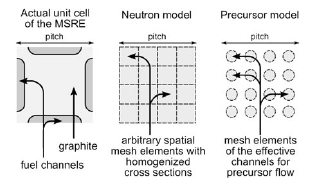
\includegraphics{kophazi_neutronics_discretization.png}
  \caption{Homogenized model of fuel channels \cite{kophazi_development_????}}
  \label{fig:kophazi_homo}
\end{figure}

\subsubsection{Thermal hydraulics}

Temperature in the fuel is determined by a 1-D convection model in the axial
direction. Moderator temperatures are calculated with a 3-D conduction
model. Coupling between the moderator and fuel temperatures is accomplished
through an axially varying heat transfer coefficient calculated with a Nusselt
correlation; see \cite{kophazi_development_????} for details of the Nusselt
correlation. Thermal expansion of the fuel was not accounted for while
determining the reactor temperature profile; however, expansion is considered
when determining homogenized neutron cross-sections.

\section{MSBR}

The most detailed report on ORNL's molten salt breeder reactor is the technical
report by Robertson. \cite{robertson_conceptual_1971} A nice overview of the
MSBR geometry is shown in \cref{fig:vertical,fig:horizontal,fig:zoom_horiz}.

\begin{figure}[htpb]
  \centering
  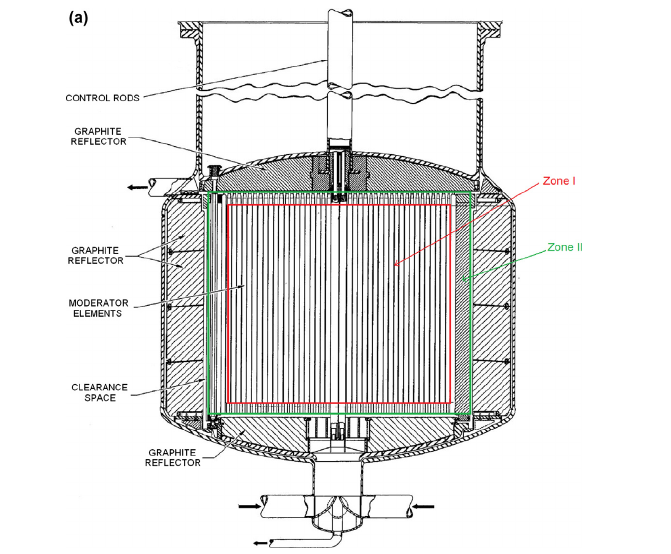
\includegraphics{vertical_MSBR_cross_section.png}
  \caption{Vertical cross section of MSBR.}
  \label{fig:vertical}
\end{figure}
\begin{figure}[htpb]
  \centering
  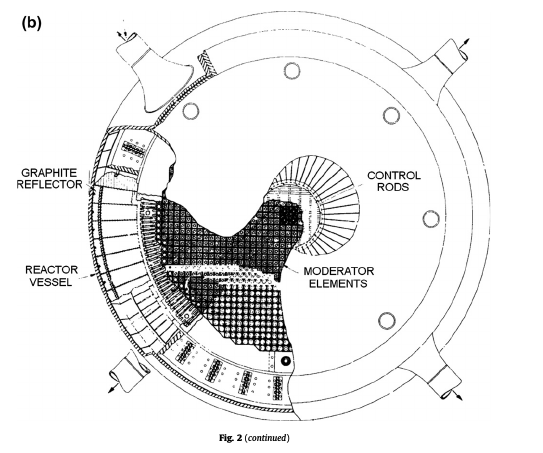
\includegraphics{horizontal_MSBR_cross_section.png}
  \caption{Horizontal cross section of MSBR.}
  \label{fig:horizontal}
\end{figure}
\begin{figure}[htpb]
  \centering
  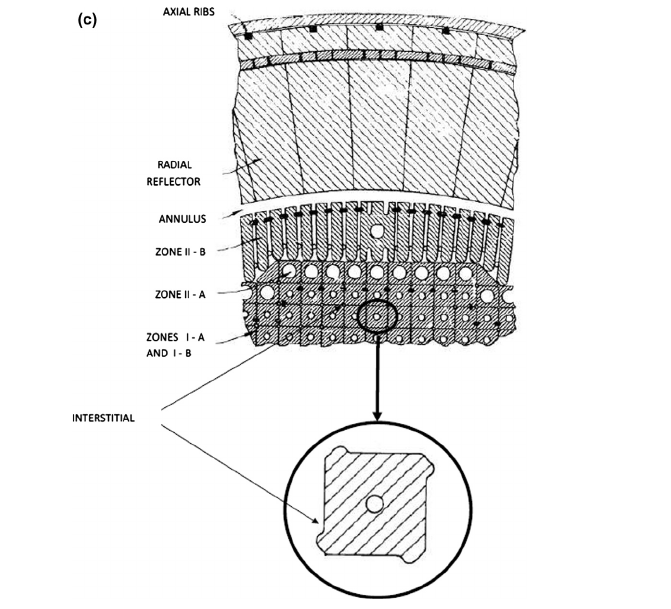
\includegraphics{zoomed_horizontal_MSBR_cross_section.png}
  \caption{Zoomed in horizontal cross-section of MSBR. Shows presence of
    interstitials between graphite block elements in zone 1 of the reactor.}
  \label{fig:zoom_horiz}
\end{figure}

\section{Simplified models}

\subsection{MSBR children}

\subsubsection{Cammi et. al.}

This model is based on the multi-physics model by
\cite{cammi_multi-physics_2011}.

Model's simplifications:
\begin{enumerate}
	\item Considered only one channel (diameter ~0.05 m)
	\item Hollow cylinder instead of block with a hole (with keeping the same fuel to graphite ratio) 
	\item Infinite length of the channel (z tends to infinity)
\end{enumerate}

\begin{figure}[htpb]
  \centering
  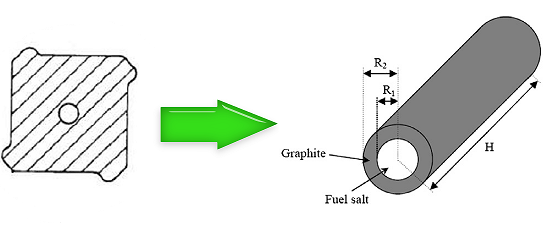
\includegraphics{Cammi_simplification_1.png}
  \caption{Cammi's simplification of MSBR's geometry. \cite{cammi_multi-physics_2011}}
  \label{fig:simlification}
\end{figure}

\FloatBarrier

\bibliographystyle{unsrt}
\bibliography{MSR-design}
\end{document}
